\subsection*{Ejercicio 5}

\begin{flushleft}
  El caso en el cual todos los elementos del vector estan ordenados el
  programa solo realiza operaciones elementales (comparaciones y
  operaciones) n-1 veces, luego la complejitud del problema será lineal.

  \begin{figure}[H]
  \centering
    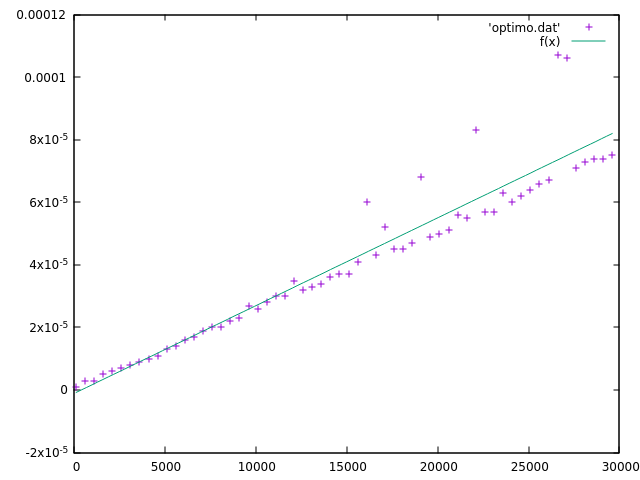
\includegraphics[width=0.8\textwidth]{resultado.png}
  \end{figure}
  
\end{flushleft}
